
% Discovery chapter ---------------------------------------------------
\chapter*{Discovery}
\addcontentsline{toc}{chapter}{Discovery}

\begin{flushright}
\parbox{0.8\textwidth}{
\emph{I don’t believe in God but I’m very interested in her. \\
\hspace*{\fill}{\textperiodcentered \textperiodcentered \textperiodcentered \hspace*{0.2em} Arthur C. Clarke} } }
\end{flushright}

\noindent
Discovery is chess variant which is played on 24 x 24 board, with
light (pastel!) yellow and gray fields and darker gray and dark teal
pieces. In algebraic notation, columns are enumerated from 'a' to 'x',
and rows are enumerated from '1' to '24'. A new piece is introduced,
Monolith.

\clearpage % ..........................................................

\section*{Monolith}
\addcontentsline{toc}{section}{Monolith}

\noindent
\begin{wrapfigure}{l}{0.4\textwidth}
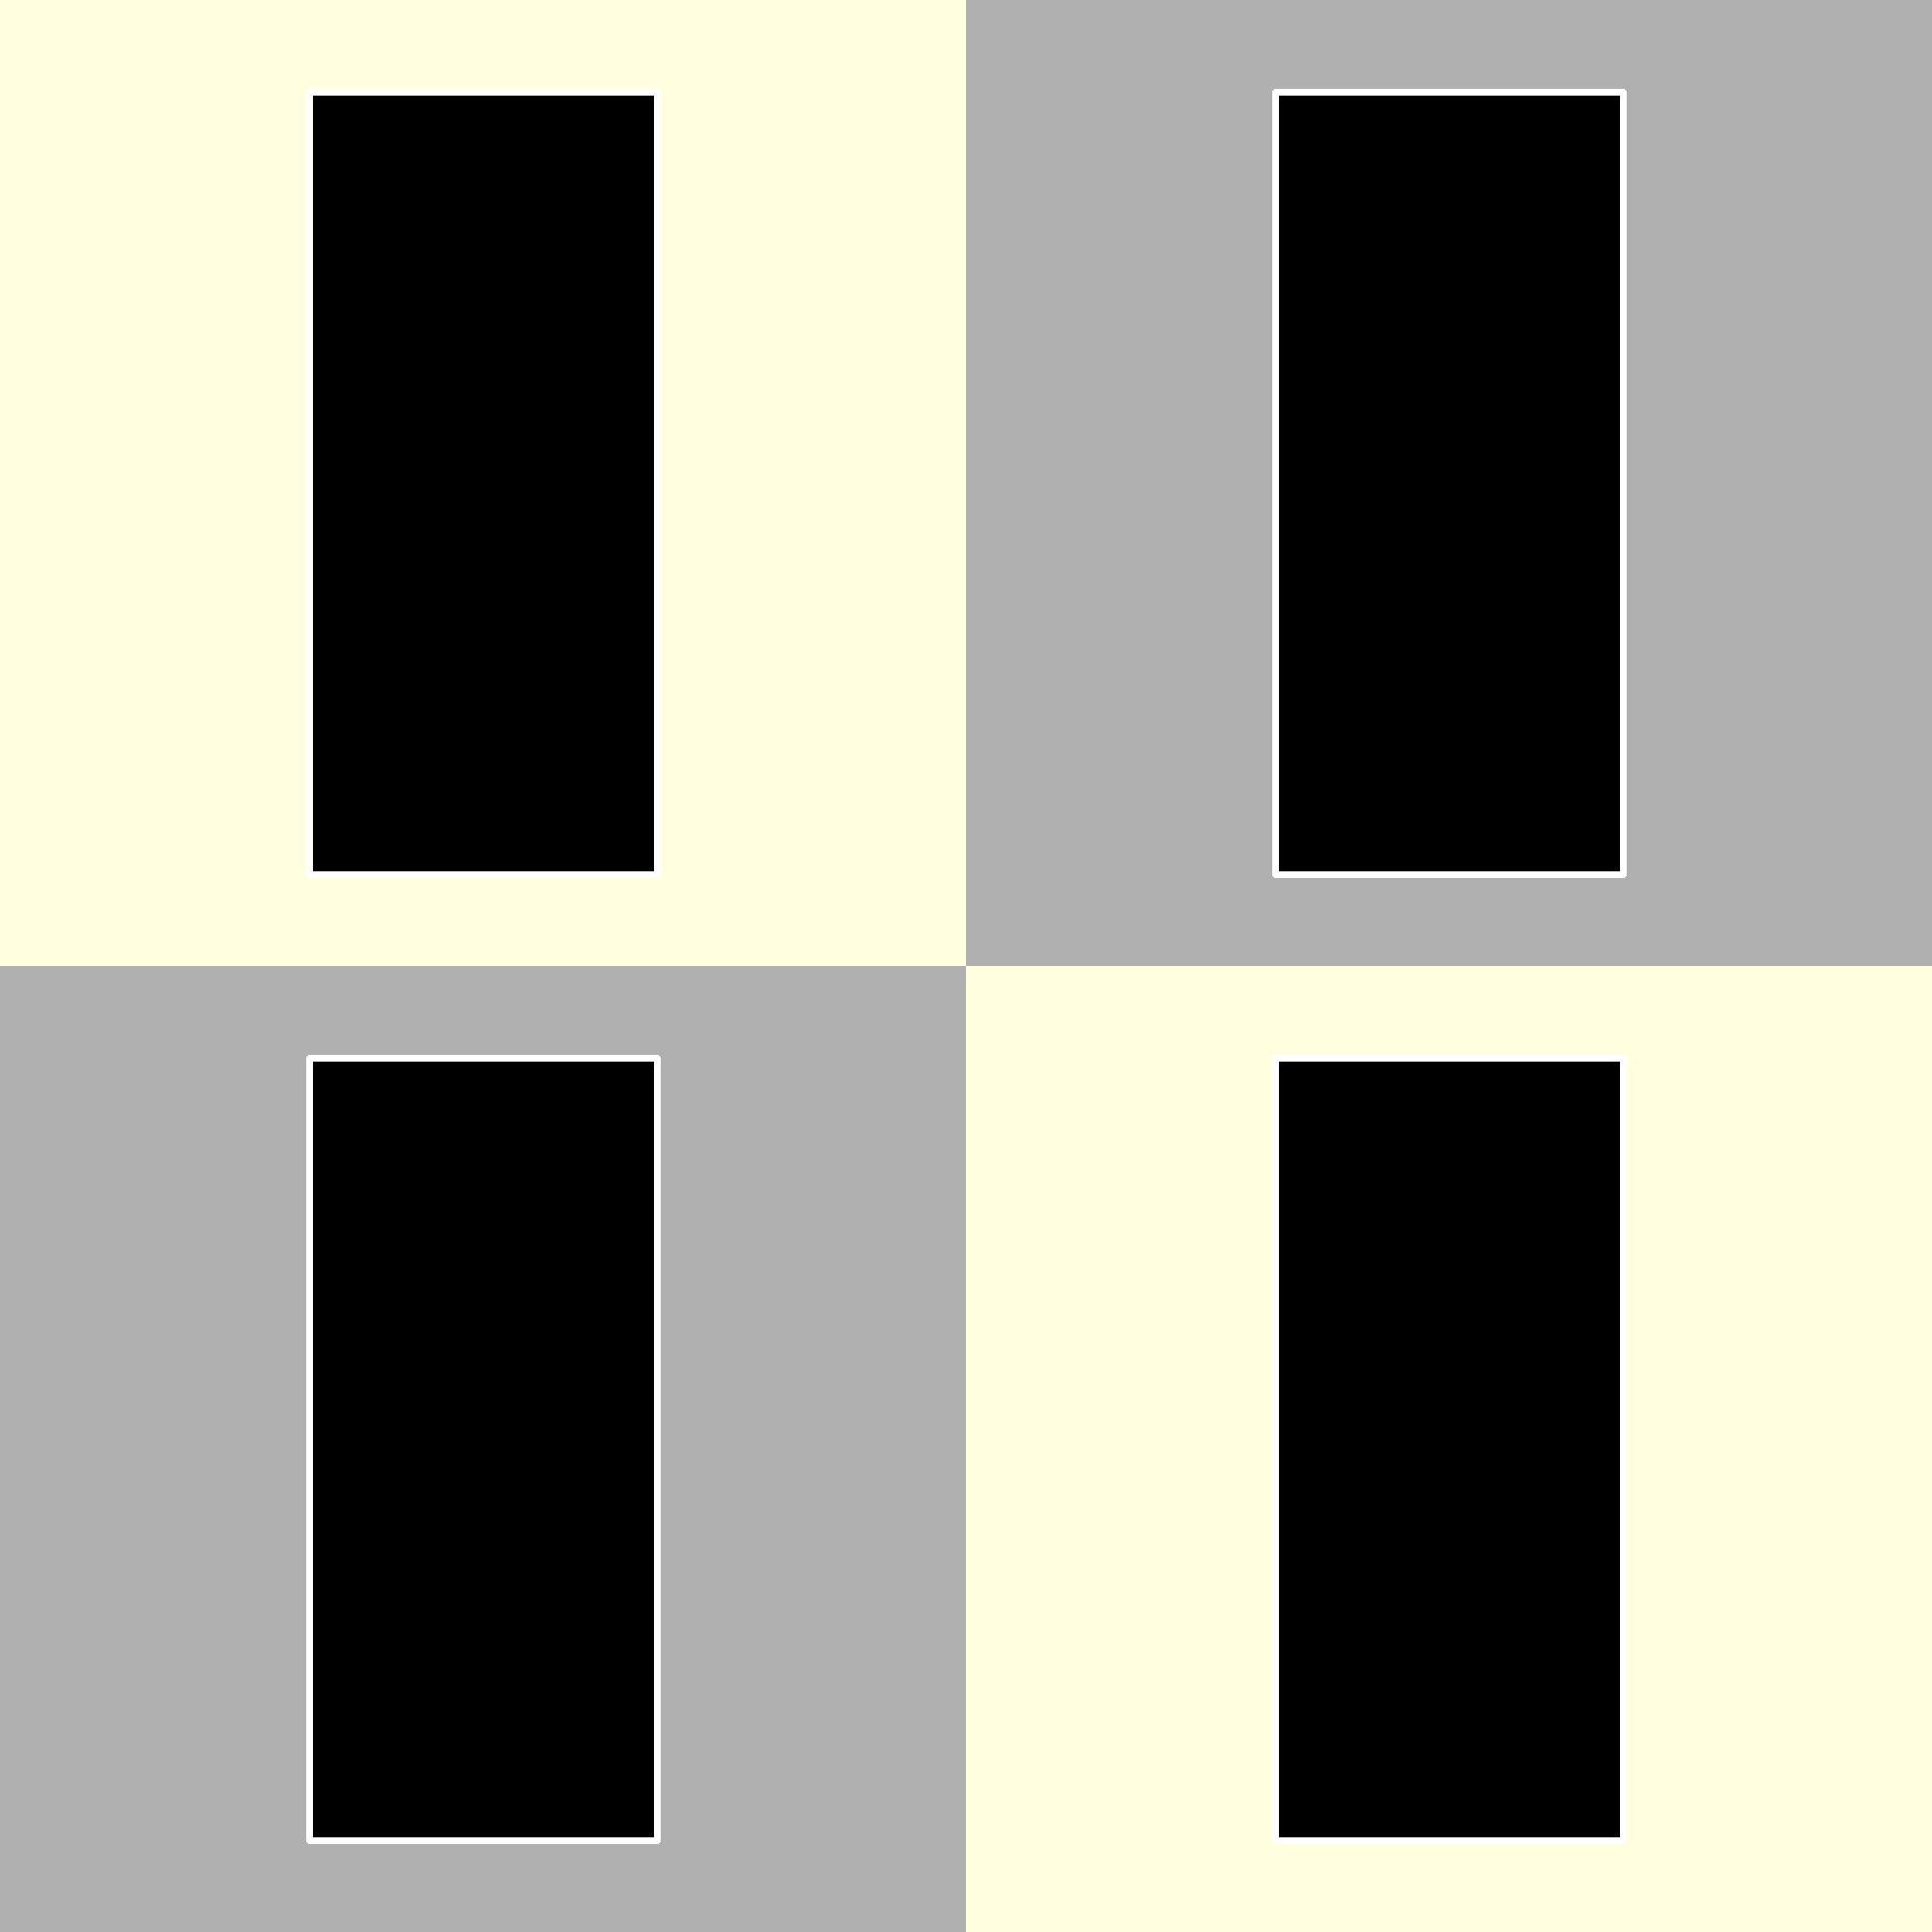
\includegraphics[width=0.4\textwidth, keepaspectratio=true]{pieces/15_monolith.png}
\caption{Monolith}
\label{fig:15_monolith}
% % \centering
\end{wrapfigure}

Pawn cannot be promoted to Monolith.

\clearpage % ..........................................................

\section*{Initial setup}
\addcontentsline{toc}{section}{Initial setup}

Initial setup can be seen in image below:

\noindent
% \begin{figure}[t]
\begin{figure}[h]
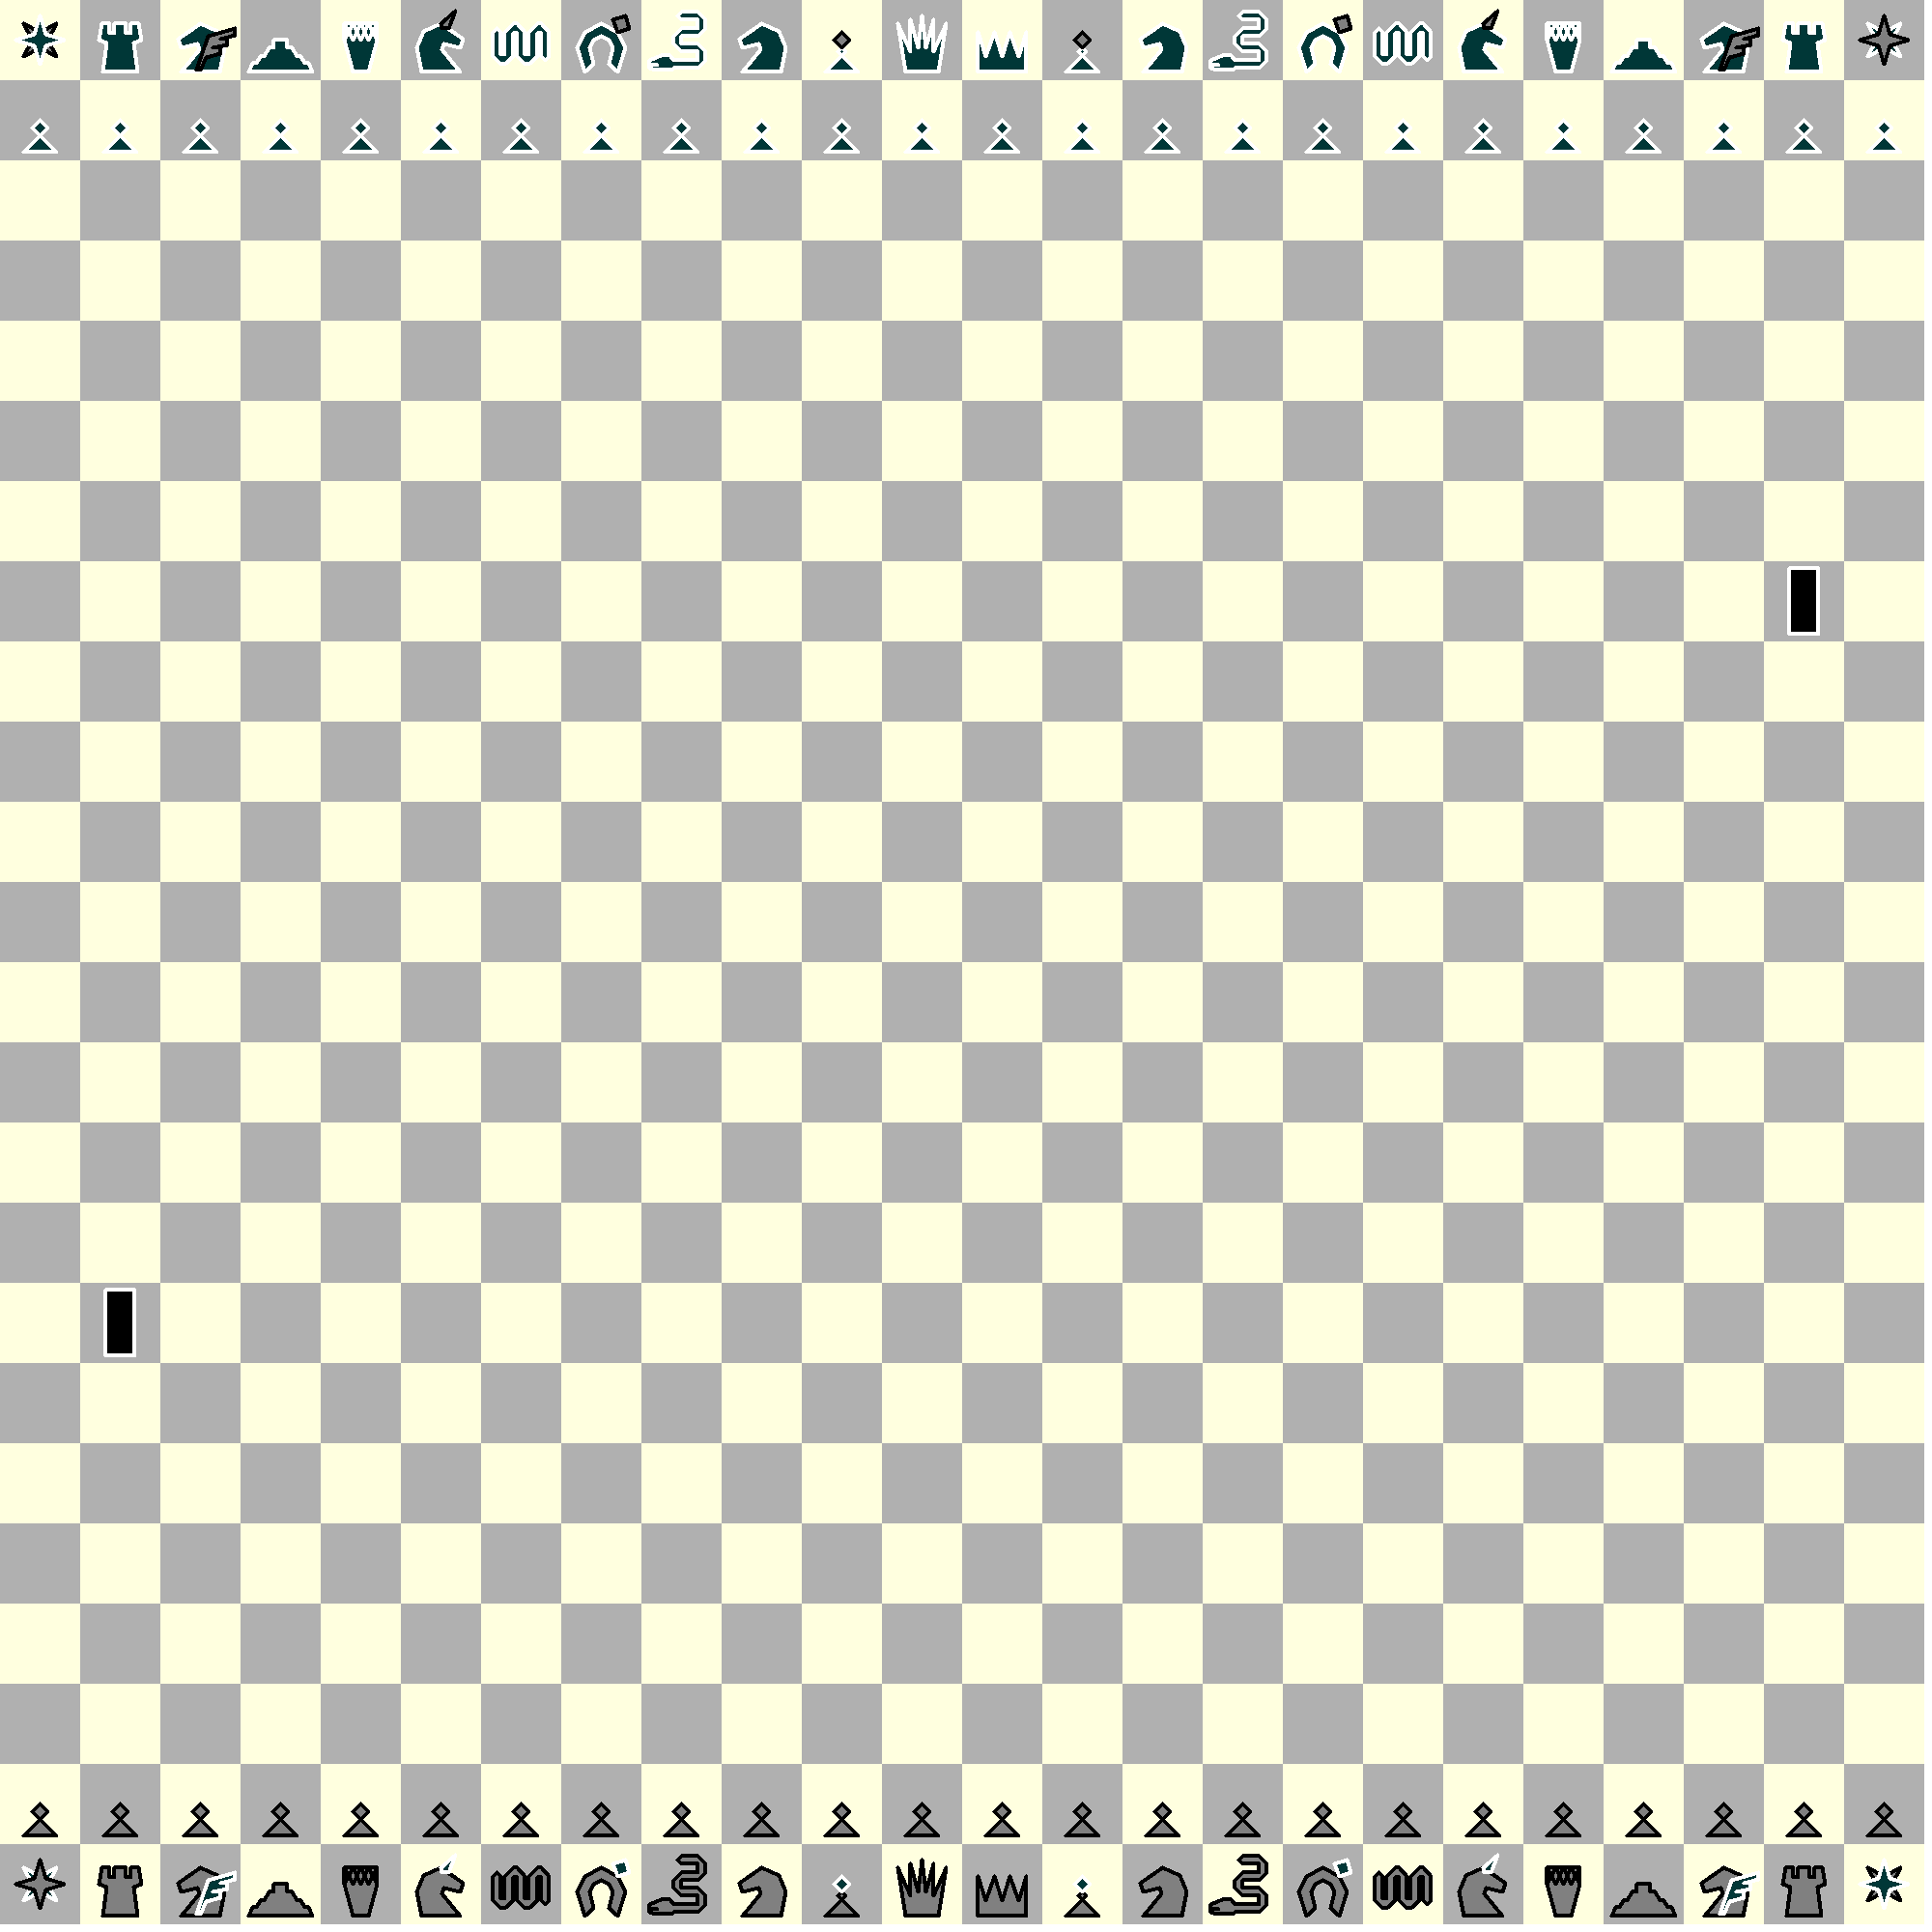
\includegraphics[width=1.0\textwidth, keepaspectratio=true]{boards/20_discovery.png}
\caption{Discovery board}
\label{fig:20_discovery}
% \centering
\end{figure}

\clearpage % ..........................................................
% --------------------------------------------------- Discovery chapter
